% !TeX spellcheck = cs_CZ
\chapter[DoS útoky]{DoS útoky}
V~této kapitole budou rozebrány DoS útoky, jejich princip, charakteristika a následně
dělení. Dále tato kapitola zmiňuje využití DDoS útoků jako služby. V~závěru jsou
zmíněny implementované útoky.

\section{Charakteristika}
DoS lze charakterizovat jako kybernetický útok, který si klade za cíl znepřístupnění
 cílové služby legitimním uživatelům. Využívají jedné nebo více zranitelností v~implementaci
 konkrétního software. Ve své podstatě každá stanice se může stát cílem, obětí, útoku
 DoS. DoS útoky se mezi útočníky velmi rychle staly populárními a tento trend
 se nemění \cite{akamai_q2_2017}. Realizace DoS útoku není nikterak obtížná a
 nevyžaduje z~útočníkovy strany hluboké znalosti, jelikož nástroje k~jejich provedení jsou
 běžně dostupné. %, viz. kapitola \ref{chap:nastroje_pro_dos}.
 Fakt, že narušit činnost sítě bývá
 jednodušší, než do ní získat přístup podporuje tento trend a jejich rozšířenost. 

Motivy takových útoků mohou být hacktivizmus, vydírání, nekalé konkurenční praktiky,
zlomyslnost nebo smokescreen coby prostředek krytí jiného současně prováděného útoku nebo
určitá forma protestu. Dalšími motivy mohou být také uznání hackerské komunity nebo také
politické politický motiv.

Velká část útoků využívá nedostatků v~architektuře rodiny protokolů TCP/IP, které byly k~tomu,
aby byly funkční, nikoliv bezpečné. Používaly se v~otevřeném a důvěryhodném prostředí, čemuž
v~dnešní době není.

Trend naznačuje rostoucí počet druhu a implementací jednotlivých útoků, proto bychom měli
věnovat pozornost a určité úsilí na ochranu proti nim. Útočník je ve výhodě, jelikož nelze
jednoznačně predikovat cíl jeho útoku.


\section{Typy útoků}
\subsection{Útok z~jednoho zdroje a útok distribuovaný}
\label{subs_ddos}
DoS útoky mohou být prováděny z~jednoho místa, což je méně časté, jelikož při
DoS útoku není útočník z~důvodu malé šířky pásma schopen vygenerovat dostatečný síťový
provoz na to, aby způsobil odepření služby na cíli svého útoku. Lze tedy jeho účinek znásobit a
to použitím většího počtu útočících stanic. Takový útok nazýváme Distributed Denial of Service (DDoS). V~případě
DoS útoku není útočník mnohdy schopen vygenerovat dostatečný síťový provoz na to, aby
způsobil odepření služby na cíli svého útoku.

Pro distribuovaný DoS útok je charakteristický velmi vysoký počet uživatelských stanic,
či serverů, použitých k~realizaci tohoto útoku. Pohybujeme se v~řádech desítek, stovek až
milionů počítačů. 
Často jsou tyto počítače napadeny virem, trojským koněm nebo programem, který v~sobě ukrývá
skrytou funkci a následně jsou zneužitý k~účelům DoS útoku bez vědomí jejich majitele.
Zajímavým cílem útočníků jsou zařízení IoT, které útočník může následně využít k~DoS
útoku.

Takové stanice nazýváme \uv{boti} a seskupení více těchto stanic \uv{botnety}. Důvody pro
vytvoření botnetu jsou větší šířka pásma, šíření spamu nebo redistribuce malware nejen do sítě,
kde se \uv{bot} nachází. Tito \uv{boti} jsou zapojeni do Command and Control (C\&C) infrastruktury spolu
s~Internet Relay Chat (IRC) servery skrze které může útočník rozesílat instrukce botům. %TODO:zdroj
IRC servery poskytují centralizovanou správu botů nebo celých botnetů skrze C\&C
mechanizmy. Jedním z mnoha trojských koní je Linux.Kaiten. Jedná se o klienta ovládaného skrze
IRC server, který může stahovat a spouštět soubory, provádět DDoS útoky za
použití UDP Flood a SYN Flood útoků a také umožňuje spoofing IP adresy.

Útoky vedené skrze tyto botnety dokáží plně zahltit šířku pásma oběti a způsobí tak odepření
služby. 
Boti mohou být rozmístěni kdekoli po světě, což znesnadňuje ochranu tím, že nelze
jednoznačně podle geolokační stopy IP adresy filtrovat provoz z~konkrétní země, což je
podpořeno možností měnit zdrojovou adresu v~IP datagramu, tzv. IP spoofing.
%TODO:obrazek utoku za pomoci spoofovane ip adresy
%http://2.bp.blogspot.com/-rYIV6yeCTeo/UI7d4414dAI/AAAAAAAAAP4/zhmngzNMKyA/s1600/b0004999_07053315.jpg
%TODO:zde vlozit obrazek ddos utoku

\subsection{Zesílené útoky}
\subsubsection{Reflektované útoky}
\label{subsec:reflektovane_utoky}
K~zesílení útoku lze použít \uv{reflektor}. Reflektor je prvek v~síti, který reflektuje provoz
iniciovaný ze strany útočníka. Při takovém útoku je \uv{spoofována} zaměněna zdrojovoá adresa
v~IP datagramu. Útočník při trojcestném handshakingu (three-way handshake) zasílá na reflektor
paket s~příznakem SYN se spoofovanou adresou, ten následně odpoví paketem s~příznakem SYN/ACK
na podvrženou IP adresu, tedy adresou oběti. Reflektor tak neodesílá odpověď útočníkovi ale
oběti. Při dostatečném počtu odeslaných žádostí směrem k~oběti dochází k~vyčerpání zdrojů, tedy
k~odepření služby. Oběť se tak může domnívat, že na ni útočí reflektory. Pravý útočník zůstává
skryt. Reflektovaný útok lze označit jako Distributed Reflection Denial of Service (DRDoS).

\subsubsection{Amplifikované útoky}
Jiným typem jsou takzvané \uv{amplifikované} útoky, které využívají \uv{amplifikátoru}.
\uv{Amplifikátor} amplifikuje, tedy zvětšuje síťový provoz zaslaný útočníkem a zasílá jej na
spoofovanou IP adresu oběti, což tento útok činí silnějším než je přímý útok. Útočník je díky
tomuto schopen vygenerovat dostatečný síťový provoz pro zahlcení oběti.

Příkladem takové amplifikace může být například dotaz na DNS server, v~jehož zóně se nachází
rozsáhlý TXT záznam. Nebo v~případě Network Time Protocol (NTP) serveru si můžeme zažádat o~posledních~600
adres, které se k~němu připojily. Následující tabulka \ref{tab:udp_ampl} zobrazuje,
kolikanásobně je větší odpověď od reflektoru oproti vyslané žádosti směrem k~němu.

\begin{table}[]
	\centering
	\caption{Amplifikační útoky založené na UDP \cite{TA14-017A}}
	\label{tab:udp_ampl}
	\begin{tabular}{|l|l|}
		\hline
		Protokol               & Faktor zvětšení šířky pásma    \\ \hline
		NTP                    & 556.9                          \\ \hline
		CharGen                & 358.8                          \\ \hline
		DNS                    & do 179                         \\ \hline
		QOTD                   & 140.3                          \\ \hline
		Quake Network Protocol & 63.9                           \\ \hline
		BitTorrent             & 4.0 - 54.3                     \\ \hline
		SSDP                   & 30.8                           \\ \hline
		Kad                    & 16.3                           \\ \hline
		SNMPv2                 & 6.3                            \\ \hline
		Steam Protocol         & 5.5                            \\ \hline
		NetBIOS                & 3.8                            \\ \hline
	\end{tabular}
\end{table}

Pro větší účinek těchto zesílených útoků lze využít namísto DoS útoku útok DDoS.

\section{Dělení útoků}
%Útoky lze také specifikovat a rozdělit podle TCP/IP vrstev, skrze které působí.
\subsection{Podle počtu útočících zařízení}

\subsection{Podle spotřeby zdrojů}

\subsection{Podle rychlosti}

\subsection{Podle spoje}
%spojované a nespojované

\section{DDoS jako služba}
Dnes uživateli běžně přístupné služby v podobě DoS nebo DDoS útoků poskytované
konkrétními službami lze nazvat Denial of Service as Service (DDoSaaS).

Definuji sebe sama jako službu stresového testování přičemž po objednateli této služby není
vyžadována znalost datových sítí. Ve smluvních podmínkách se zříkají odpovědnosti za škody
způsobené objednateli. Přičemž ani nezjišťují, zda cíl útoku, který si zákazník objednal je či
není v jeho správě. Vyžadují registraci a za úplatu poskytují stresové testování. Platbu je
možno provádět buď v Bitcoinech nebo přes PayPal. Ceny za tuto službu se pohybují přibližně v
rozmezí mezi 2-10 americkými dolary. Mnoho takových služeb nabízí i podporu typu 24/7 skrze
Instant messaging (IM). Dostupných bývá povětšinou pár základních útoků založených na protokolech
Transmission Control Protocol (TCP), User Datagram Protocol (UDP) a Hypertext Transfer Protocol (HTTP). Tyto služby využívají také IP spoofing
a zesílení útoku pomocí amplifikátorů \ref{subsec:reflektovane_utoky}. 

Největší hrozbou DDoSaaS útoků je jejich snadná dostupnost. Avšak tyto útoky nejsou
nikterak sofistikované a nejsou příliš velkou hrozbou pro standardně zabezpečenou síť
\cite{DDoSaaS}.

\section{Útoky mířené na síťové zdroje}
Cílem tohoto útoku je zaplavit celou síť množstvím paketů tak, aby byla spotřebována většina
šířky pásma konkrétní sítě. Při těchto útocích je obvyklé použití botnetu při jeho samotném
vykonávání.

\subsection{Záplavové}
\label{subs_zaplavove}
Nejběžnější jsou útoky, které používají protokol UDP, který je nespojovaný, nepotvrzovaný a
bezstavový. Toto jej činí ideálním pro tento typ útoku. Protokol UDP na rozdíl od TCP
nevyžaduje sestavení spojení, tzv. třícestný handshaking, to útočníkovi dovoluje podvržení
IP adresy. Při záplavovém útoku útočník zasílá velké množství UDP paketů a volí náhodné
cílové porty a také IP adresy. Server, oběť, je tak nucen odpovídat na každou takovou
přijatou zprávu odpovídat zprávou ICMP (Destination unreachable - \uv{Cíl nedosažitelný}),
čímž spotřebuje velkou šířku pásma a dochází tak k DoS útoku.

%TODO obrázek UDP floodu

Podobným útokem je ICMP Flood, při němž útočník posílá oběti zprávu \uv{Echo request} a oběť
na každou takovou musí odpovídat zprávou \uv{Echo reply}, spotřebovává tak velkou šířku
pásma a dochází k DoS útoku.
Záplavové útoky jsou efektivnější v případě použití botnetu, tudíž DDoS útoku.

%TODO \section{Útoky mířené na serverové zdroje}
% jak funguje normalne, slabina v tcp/ip, pomale utoky

\section{Útoky mířené na aplikační zdroje}
Tyto typy útoků se zaměřují na zranitelnosti samotné aplikace využívající protokoly 
7. vrstvy ISO/OSI modelu. Využívají zranitelností v implementaci samotného aplikačního
protokolu nebo aplikace běžící na cílovém serveru. Tato zranitelnost nemusí nutně býti
implementační chybou ale jen slabým místem, kterého lze využít. Takovým může být kupříkladu
situace, kdy vyšleme na server požadavek, jež je na straně serveru nutno zpracovat, čímž
server spotřebuje velké množství výpočetních zdrojů. Je-li takovýchto příchozích žádostí na
server vysláno více, dochází na jeho straně k vyčerpání výpočetních zdrojů, nelze zpracovat
požadavky legitimních uživatelů, čímž dochází k odepření služby a tedy k úspěšnému DoS útoku.

Tyto útoky využívají nejen záplavovou \ref{subs_zaplavove} techniku, ale i pomalou, kterou je
kupříkladu Slowloris.
 
Příkladem takových útoků může být HTTP GET Flood, který je prováděn povětšinou botnetem, kdy
se útočník snaží ze serveru získat kořenovou stránku nebo objemný soubor umístěný na této
stránce. Server je nucen odesílaný obsah zkopírovat do své paměti a neuvolnit jej po dobu
trvání spojení, potažmo útoku, čímž v paměti nezbývá místo na legitimní požadavky běžných
uživatelů.

Dalším útokem, který cílí na aplikační zdroje je Slowloris, který využívá techniky pomalého
útoku. Útočník se serverem standardně naváže TCP spojení a oznámí serveru nízkou nebo nulovou
velikost okna.

Takových spojení vytvoří co nejvíce a snaží se je udržet otevřená po co nejdelší dobu.
Server pak útočníkem požadovaná data rozdělí do většího poctu menších častí v závislosti na
velikosti okna. V případě více takových spojení je server zaneprázdněn po dlouhou dobu a
další navázání dalších spojení odmítá, čímž se stává nedostupným a dochází tedy k DoS
útoku.

Do této kategorie útoků lze zařadit taky útoky na protokoly DNS, SMTP, SNMP a další.
%slow read?

\section{Implementované útoky}
V této kapitole jsou rozebrány útoky, které byly implementovány do aplikace DoSGen.

\subsection{NTP flood}
%http://www.ntp.org/documentation.html
%https://www.csirt.cz/page/2793/prevence-zneuziti-ntp-k-ntp-amplification-utokum/
%TODO schéma útoku
Protokol aplikační vrstvy, NTP slouží k synchronizaci času mezi stanicemi v síti.
Využívá protokol UDP a komunikuje na portu 123.

Tento útok se zaměřuje na zneužití příkaz monlist, která vrací seznam IP adres
posledních 600 klientů připojených k NTP serveru. Primárně tento příkaz slouží k
monitorování provozu na serveru. Dotaz s kódem žádosti 42 \uv{MON\_GETLIST\_1}  můžeme vidět
na obr.  \ref{fig:monlist_get_wireshark-img}. Útočník se tedy zaměřuje na získání co
největší amplifikace, tedy toho, aby odpověď zaslaná na podvrženou IP adresu oběti
byla několikanásobně větší než dotaz zaslaný ze strany útočníka. NTP server však
nedokáže identifikovat, zda je či není zdrojová adresa podvržena.
Tento útok lze kategorizovat jako amplifikační útok, kde amplifikací je právě odpověď
NTP serveru, kterou provádí funkce monlist.

%obrazek-screen wireshark
\begin{figure} [ht]
	\centering
	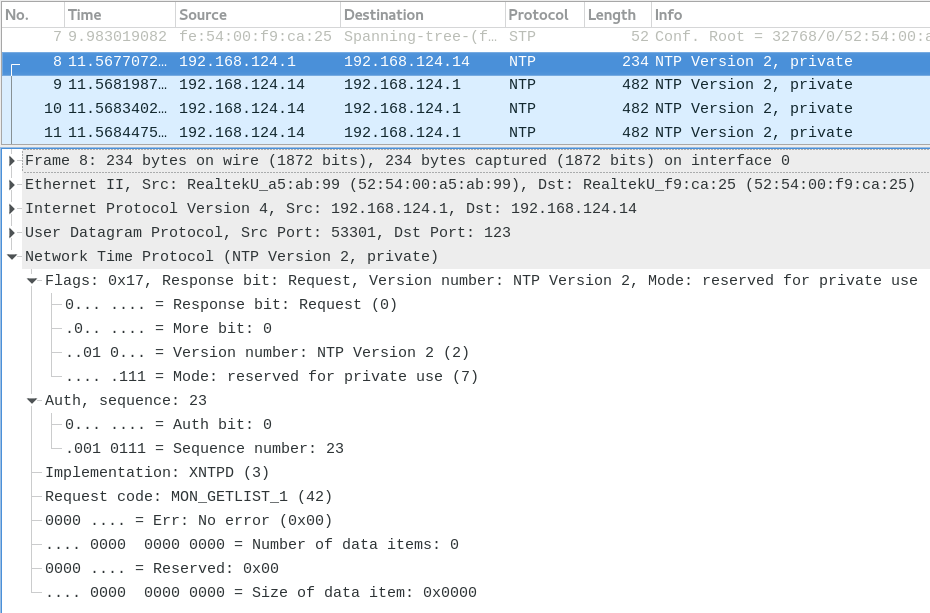
\includegraphics[width=0.9\textwidth]{obrazky/mon_getlist_1_wireshark.png} %.pdf
	\caption{Dotaz na NTP server s kódem žádosti 42 - monlist}
	\label{fig:monlist_get_wireshark-img}
\end{figure}

Útočníci si průběžně mapují NTP servery, které lze takto zneužít a použijí je k 
DDoS útoku.
Oběť je tak zahlcena provozem ze všech těchto NTP serverů a nezbývá dostatek šířky
pásma pro komunikaci s legitimními uživateli (klienty), pro které se tak služba běžící na
serveru, který se stal obětí, stane nedostupnou. Dochází tedy k odepření služby a úspěšnému
DDoS útoku.

To, zda je náš server zranitelný lze zjistit pomocí příkazu \texttt{ntpdc}\footnote{Příkaz
\texttt{ntpdc} je ve verzi ntp-4.2.8 zastaralý, používá se \texttt{ntpq} jako náhrada.}.
Vrací-li nám server odpověď, je zranitelný. Následující ukázka demonstruje právě zmíněné.
Výstup příkazu \texttt{ntpdc} je zkrácen na prvních deset řádků výstupu a ořezán zprava o
tři sloupce, a to o \uv{rstr}, \uv{avgint} a \uv{lstint}. Ve druhém příkazu lze vidět, že
server nám vrací 600 záznamů nepočítaje první dva řádky výpisu.


%ntpdc výstup, ukázka počtu záznamů
\lstinputlisting[language=bash]{code/ntpdc_monlist.sh}

Nejjednodušší ochranou proti tomuto útoku je aktualizace NTP serveru na verzi 4.2.7p26, kde
je příkaz \texttt{monlist} zcela odstraněn. Chceme-li zůstat na aktuální verzi NTP serveru,
je nutno změnit konfiguraci v souboru \texttt{/etc/ntp.conf}, a to přidáním direktivy
\texttt{noquery} do řádku začínajícího slovy \uv{\texttt{restrict default}} a následně přidáním
\texttt{disable monitor} na nový řádek konfiguračního souboru. 
Celá tato zranitelnost byla popsána v CVE-2013-5211. %TODO citovat CVE

Balíček NTP serveru pro některé distribuce již v prvotní čisté instalaci obsahuje korektně
nastavený konfigurační soubor. Například v systémech RHEL a Fedora byla tato direktiva
přítomna dlouho před vydáním tohoto CVE. %TODO citovat specfile nebo bugzillu?
